\chapter{OpenAI Gym}

OpenAI Gym je Python biblioteka \engl{library} otvorenog koda \engl{open source} koja služi za razvijanje i usporedbu agenata u odabranim okolinama. Iznimno je popularna u sferi simpatizera i programera koji se bave razvijanjem modela podržanog učenja zbog jednostavnosti korištenja, velikog broja dostupnih okolina i jednostavnog stvaranja novih okolina, te jednostavne interakcije agenta i okoline. OpenAI Gym biblioteka se redovito održava i trenutno je na verziji \texttt{0.24.1}. 

\section{Struktura}

Interakcija agenta i okoline podijeljena je na epizode. Na početku svake epizode, početno stanje se nasumično uzorkuje iz distribucije, i interakcija se nastavlja sve dok se okolina ne nađe u terminalnom stanju \cite{OpenAIWhitepaper}.

\begin{listing}[H]
    \caption{Jednostavan primjer integracije agenta i Gym okoline (1 epizoda)}
    \inputminted{python}{snippets/init.py}
    \label{lst:init-code}
\end{listing}

Prikazan je potpuno funkcionalni kod \ref{lst:init-code} koji reprezentira jednostavnu interakciju agenta i okoline. Agent u ovom jednostavnom slučaju nasumično odabere akciju iz skupa svih dostupnih akcija za tu okolinu (linija 9). Osnovni kostur se sastoji od koraka specifikacije okoline (linija 3), inicijalizacije okoline (linija 5) te interakcija okoline i agenta - agent predaje okolini odabranu akciju, okolina vraća povratnu informaciju (linije 7 - 14). 

\begin{figure}[h]
    \centering
    \frame{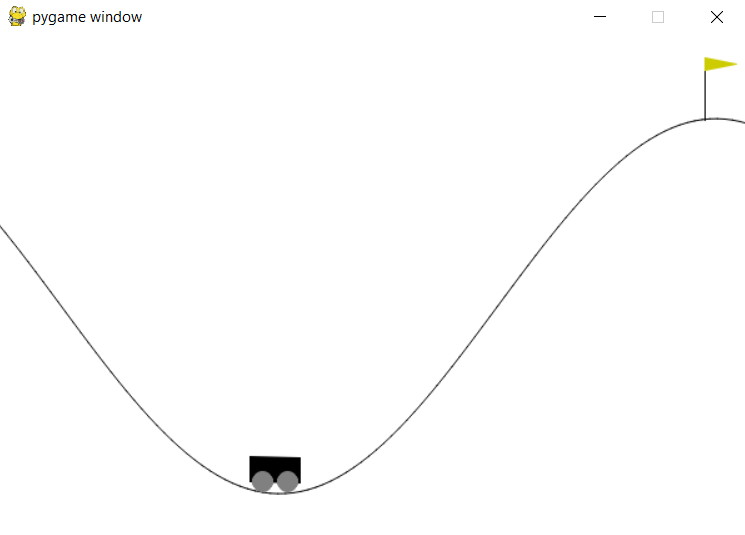
\includegraphics[width=10cm]{assets/mountain-car.png}}
    \caption{Rezultat pokretanja koda \ref{lst:init-code}}
    \label{fig:mountain-car}
\end{figure}

\subsection{Okolina}

Temelj oko kojeg se zasniva OpenAI Gym biblioteka jest razred \engl{class} \texttt{Env} koji u suštini implementira simulator koji pokreće okruženje u kojem naš agent može interaktirati s okolinom. Točnije rečeno, enkapsulira sva potrebna ponašanja i metode koje su potrebne za jednostavnu interakciju. Objekt tipa \texttt{Env} stvara se pozivanjem funkcije \texttt{gym.make()} (kod \ref{lst:init-code} linija 3) kojoj se predaje identifikator okoline (\texttt{id}) zajedno s opcionalnim argumentima (metapodatcima). 

\subsection{Interakcija s okolinom}

Kao što je vidljivo iz koda \ref{lst:init-code} osnovne metode koje se pozivaju nad instancom razreda \texttt{Env} su \texttt{reset} i \texttt{step}. Funkcija \texttt{reset} postavlja okruženje u početno stanje i vraća njegovu vrijednost (kod \ref{lst:init-code}. linija 5). S druge strane, funkciji \texttt{step} (kod \ref{lst:init-code}. linija 10) predaje se jedna od ispravnih akcija koja inicira prijelaz okoline iz jednog stanja u drugo. Funkcija vraća 4 vrijednosti: vrijednost prostora stanja \engl{observation}, iznos nagrade kao rezultat poduzimanja određene akcije  \engl{reward}, zastavicu koja signalizira jesmo li došli u završno stanje okoline \engl{done}, te neke dodatne informacije.

Još jedna vrlo često korištena funkcija jest \texttt{render} (kod \ref{lst:init-code}. linija 12) koja služi kako bi se u određenom formatu prikazala okolina. Dostupni formati su: \texttt{human} (otvara se skočni prozor sa slikom stanja okoline - slika \ref{fig:mountain-car}), \texttt{rgb_array} (\texttt{numpy} array RGB vrijednosti) i \texttt{ansi} (string reprezentacija okoline).

\subsection{Prostor akcija i prostor stanja}

Osnovna struktura okruženja opisana je atributima \texttt{observation_space} i \texttt{actio\-n_space} koji su dio razreda \texttt{Env} i čija se vrijednost može razlikovati zavisno o okolini. Atribut \texttt{action_space} opisuje numeričku strukturu svih legitimnih akcija koje se mogu izvesti nad određenom okolinom. S druge strane, atribut \texttt{observation_s\-pace} definira strukturu objekta koje predstavlja opis stanja u kojem se okolina nalazi.

Format validnih akcija i stanja okoline, odnosno struktura tih podataka, definirana je razredima \texttt{Box}, \texttt{Discrete}, \texttt{MultiBinary} i \texttt{MultiDiscrete}. Svi navedeni razredi nasljeđuju i implementiraju glavne metode nadrazreda \texttt{Space}. 

Razred \texttt{Box} predstavlja strukturu podataka u kontinuiranom n-dimenzionalnom prostoru. Prostor i njegove validne vrijednosti omeđene su gornjim i donjim granicama koje se jednostavno postave pri inicijalizaciji strukture pridruživanjem željenih vrijednosti atributima \texttt{high} i \texttt{low}. Kod \ref{lst:box-code} prikazuje inicijalizaciju \texttt{Box} strukture podataka koja je sastavljena od \texttt{3}-dimenzionalnog vektora čije su vrijednosti omeđene odozdo i odozgo vrijednostima \texttt{-1} i \texttt{-2}. Metoda \texttt{sample(self)} nasumično uzorkuje element iz prostora koristeći različite distribucije ovisno o ograničenjima prostora.

\begin{listing}[H]
    \caption{Primjer korištenja strukture kontinuiranog prostora \texttt{Box}}
    \inputminted{python}{snippets/box.txt}
    \label{lst:box-code}
\end{listing}

Razred \texttt{Discrete} s druge strane, predstavlja strukturu podataka u diskretnom n-dimenzionalnom prostoru gdje su validne vrijednosti sve cjelobrojne vrijednosti unutar intervala $[0, n-1]$ (početna vrijednost se može specificirati). Kod \ref{lst:discrete-code} prikazuje inicijalizacije \texttt{Discrete} strukture podataka ovisno o specificiranoj početnoj vrijednosti.

\begin{listing}[H]
    \caption{Primjer korištenja strukture diskretnog prostora \texttt{Discrete}}
    \inputminted{python}{snippets/discrete.txt}
    \label{lst:discrete-code}
\end{listing}

\subsection{Omotači}

Omotači \engl{Wrappers} su prikladne strukture koje omogućavaju izmjenu elemenata postojećeg okruženja bez potrebe za mijenjanjem originalnog koda. Omotači omogućavaju modularnost, mogu se implementirati prema vlastitim potrebama i ulančavati. Ova funkcionalnost vrlo se često koristi u situacijama kada pri treniranju modela želimo normalizirati ulaze (skalirati piksele slike), provesti regularizaciju (podrezivanje vrijednosti nagrade), transformirati ulaze u Pytorch dimenzije, implementirati preskakanje slikovnih okvira...  Navedene funkcionalnosti moguće je postići tako da definiramo vlastiti omotač koji će nasljeđivati ili obični \texttt{Wrapper} nadrazred ili specifičnije razrede poput \texttt{ObservationWrapper}, \texttt{RewardWrapper}, \texttt{ActionWrapper}...

\subsection{Vektorizirana okruženja}

Koristeći standardne metode stvaranja i interakcije s Gym okruženjem, pokrećemo samo jednu instancu okruženja i na taj način ne iskorištavamo potpuno računalnu snagu koja nam je dostupna. Vektorizirana okruženja \engl{Vectorized environments} su okruženja koja paralelno pokreću više kopija istog okruženja u svrhu poboljšanja učinkovitosti i ubrzanja procesa učenja agenta.

?? TODO nastaviti ovo jer su sada objavili novu verziju u kojoj je već u Gym-u ukomponiran Vector API a ja sam do sada bio koristio njihov library \textit{baselines}. ?? - ponovna implementacija i usporedba

\begin{figure}[H]
    \centering
    \frame{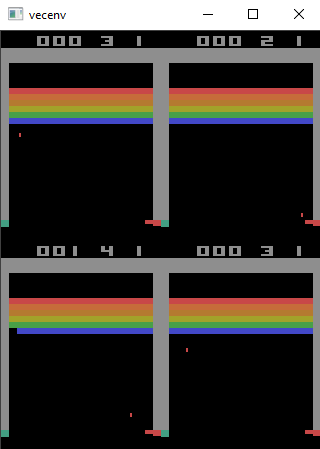
\includegraphics[height=9cm]{assets/breakout-vect.png}}
    \caption{Vektorizirano okruženje sa 4 paralelne asinkrone instance}
    \label{fig:breakout-vect}
\end{figure}

\section{Okruženja}

U OpenAI Gym ekosustavu dostupno je puno okruženja koja omogućuju interakciju s agentom. Neki od njih su: \textit{Atari} - skup od Atari 2600 okolina, \textit{MuJoCo} (punim nazivom \textit{Multi-Joint dynamics with Contact}) - skup okolina za provođenje istraživanja i razvoja u robotici, biomehanici, grafici i drugim područjima gdje je potrebna brzina i točna simulacija, \textit{Classic Control} - skup okolina koje opisuju poznate fizikalne eksperimente. Opisat ćemo neke od najkorištenijih okolina.

Upravljanje agentima i njihovo izvođenje akcija u određenoj atari okolini interno je implementirano koristeći objektno orijentiranu razvojnu cjelinu \engl{framework} \textit{The Arcade Learning Environment} (skraćeno \textit{ALE}). Na taj način razdvajaju se slojevi emulacije okruženja (koristeći Atari 2600 emulator \textit{Stella}), sloj koji kontrolira samog agenta \textit{(ALE)} i sloj koji pruža jednostavnu programsku implementaciju i interakciju \textit{(OpenAI Gym)}\cite{OpenAIALE}. 

TODO stohastika i determinizam u atariu (frame skipping, repeat action...) - https://www.gymlibrary.ml/environments/atari/

\subsection{Okruženje CartPole}

Ovo okruženje modelira fizikalni problem održavanja ravnoteže. Inačica je sličnog fizikalnog problema pod nazivom \textit{obrnuto njihalo} \engl{inverted pendulum}. Za pomična kolica zakvačen je stupić. Njegovo težište nalazi se iznad središta mase i na taj način osigurava da sustav nije stabilan.  Zglob, odnosno dodirna točka između stupića i kolica nema trenja niti drugih gubitaka. Također, kolica koja se kreću vodoravno po putanji u 2 smjera nemaju trenja niti drugih gubitaka. Cilj ovog fizikalnog problema jest uravnotežiti stup primjenom sila i pomicanjem kolica u lijevom ili desnom smjeru.

Za svaki poduzeti korak okolina dodjeljuje nagradu u vrijednosti $+1$. Struktura valjanih akcija koje agent može poduzeti (\texttt{action_space}) instanca je razreda \texttt{Disc\-rete(2)} - skup akcija je diskretan i u svakom koraku je moguće odabrati 1 od maksimalno 2 dostupne akcije. Opis značenja svake akcije prikazan je u tablici \ref{table:cart-pole-action}. S druge strane, objekt koji predstavlja strukturu stanja okoline u određenom vremenskom trenutku (\texttt{observation_space}) instanca je razreda \texttt{Box(4)} – stanje se sastoji od 4 kontinuirane vrijednosti od kojih su neke ograničene i odozdo i odozgo. Točan opis i granice vrijednosti predočeni su u tablici \ref{table:cart-pole-observation}.

\begin{table}[ht]
    \centering
    \caption{Opis valjanih akcija okoline CartPole - atribut \texttt{action_space}}
    \begin{tabular}{c c}
        \toprule
        Akcija & Opis akcije  \\
        \midrule
        0 & Pomak kolica ulijevo \\
        1 & Pomak kolica udesno \\
        \bottomrule
    \end{tabular}
    \label{table:cart-pole-action}
\end{table}

\begin{table}[ht]
    \centering
    \caption{Opis strukture okoline okoline CartPole - atribut \texttt{observation_space}}
    \begin{tabular}{c c c c}
        \toprule
        Indeks & Opis & Donja granica & Gornja granica \\
        \midrule
        0 & Pozicija kolica & $-4.8$ & $4.8$ \\
        1 & Brzina kolica & $-\infty$ & $\infty$ \\ 
        2 & Nagib štapića i kolica & $-0.418 \text{rad}$ & $0.418 \text{rad}$ \\
        3 & Brzina štapića na vrhu & $-\infty$ & $\infty$ \\
        \bottomrule
    \end{tabular}
    \label{table:cart-pole-observation}
\end{table}

Početno stanje okoline inicijalizira se pozivom metode \texttt{reset()} slučajnim vrijednostima iz uniformne razdiobe na intervalu $\pm 0.05$. Okolina podržava 3 uvjeta zaustavljanja (uvjeti koji označuju da je riječ o terminalnom stanju): nagib štapića i kolica je izvan intervala $\pm 0.2095 \text{rad}$, pozicija sredine kolica je izvan intervala $\pm 2.4$ (sredina kolica dotiče rub vidljivog prostora) i duljina epizode je veća od $500$ koraka. Na slici \ref{fig:cart-pole} prikazana je okolina CartPole zajedno s vrijednostima okoline. % TODO napraviti svoje koje bolje izgleda

\begin{figure}[H]
    \centering
    \frame{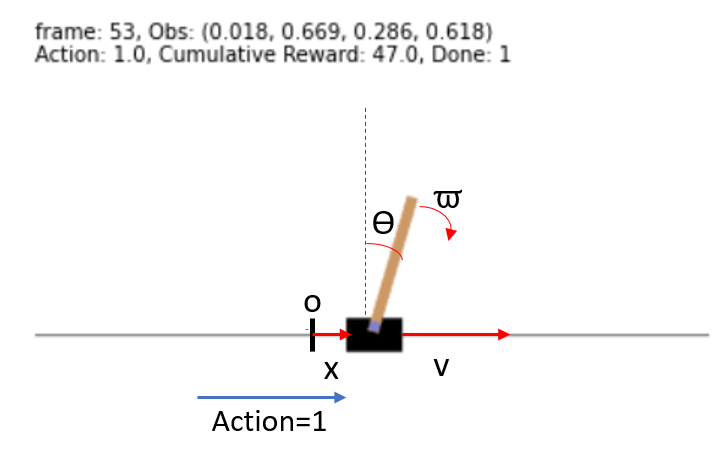
\includegraphics[height=5.5cm]{assets/cart-pole-not-mine.png}}
    \caption{Izgled i vrijednosti CartPole okoline - TODO}
    \label{fig:cart-pole}
\end{figure}

\subsection{Okruženje Breakout}

Ova okolina simulira poznatu Atari 2600 igru u kojoj je cilj sakupiti što više bodova pomičući platformu i održavajući lopticu na ekranu. Platforma je postavljena na dnu ekrana, na fiksnoj visini i moguće ju je pomicati u dva smjera. Loptica se odbija između zidova, platforme i 6 razina \textit{ciglenih} blokova čijim razbijanjem se sakupljaju bodovi. Ako loptica padne ispod platforme koju igrač kontrolira, gubi se život. Igra završava kada igrač potroši 5 života, odnosno kada 5 puta loptica padne ispod platforme. 

Skup validnih akcija je instanca razreda \texttt{Discrete(4)} - skup akcija je diskretan i u svakom koraku je moguće odabrati 1 od maksimalno 4 dostupne akcije. Opis značenja svake akcije prikazan je u tablici \ref{table:breakout-action}. Kao opis trenutnog stanja okoline moguće je dobiti RGB vrijednosti svakog piksela slike (slike dimenzije $210 \times 160$) ili vrijednosti radne memorije \textit{ALE} okoline (128 bajta) - što je korisno jer možemo preskočiti korak učenja reprezentacije okoline (preskačemo dio gdje algoritmi učenja moraju iz piksela slike naučiti reprezentaciju). Razlike u strukturi objekta okoline prikazane su u tablici \ref{table:breakout-observation}. 

\begin{table}[ht]
    \centering
    \caption{Opis valjanih akcija okoline Breakout - atribut \texttt{action_space}}
    \begin{tabular}{c c c}
        \toprule
        Akcija & Opis akcije & Detaljniji opis akcije  \\
        \midrule
        0 & NOOP & Ne poduzima se nikakva akcija \\
        1 & FIRE & Akcija koja pokreće igru \\ 
        2 & RIGHT & Platforma se pomiče udesno \\ 
        3 & LEFT & Platforma se pomiče ulijevo  \\
        \bottomrule
    \end{tabular}
    \label{table:breakout-action}
\end{table}

\begin{table}[H]
    \centering
    \caption{Opis strukture objekta okoline Breakout - atribut \texttt{observation_space}}
    \begin{tabular}{c c}
        \toprule
        Indeks & Struktura  \\
        \midrule
        RAM vrijednosti & \texttt{Box(0, 255, (128,), uint8)}  \\ 
        Vrijednosti RGB slike & \texttt{Box(0, 255, (210, 160, 3), uint8)}  \\
        \bottomrule
    \end{tabular}
    \label{table:breakout-observation}
\end{table}

Nagrada dolazi u obliku bodova koji se dobivaju uništavajući \textit{ciglene} blokove. Vrijednost nagrade ovisi o boji cigle. Izgled same okoline prikazan je na slici \ref{fig:breakout}.

\begin{figure}[H]
    \centering
    \frame{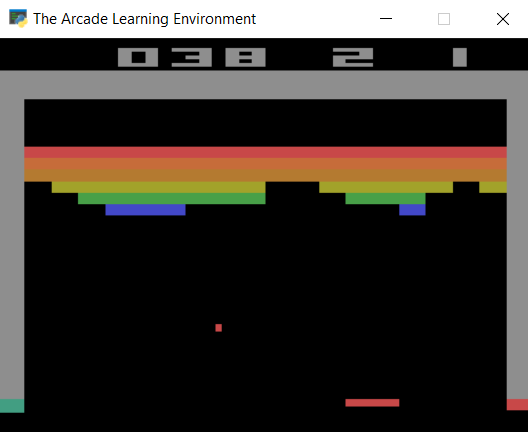
\includegraphics[width=10cm]{assets/breakout.png}}
    \caption{Okolina Breakout}
    \label{fig:breakout}
\end{figure}


% TODO dodati za literaturu https://blog.paperspace.com/getting-started-with-openai-gym/ i https://www.gymlibrary.ml/content/vector_api/ i https://www.gymlibrary.ml/ općenito

% TODO dodati za literaturu https://atariage.com/manual_html_page.php?SoftwareID=889

% značenje pojedinih ram pozicija https://github.com/mila-iqia/atari-representation-learning/blob/master/atariari/benchmark/ram_annotations.py

% https://stackoverflow.com/questions/45207569/how-to-interpret-the-observations-of-ram-environments-in-openai-gym